\section{EAC}
\label{sec:eac results}

This section will present thorough results concerning several characteristics related to the EAC method.
These were the timings of the different parts, how cardinality and the different $K_{min}$ rules affected the sparsity of the co-association matrix, the typical number of associations per cluster in each rule, the growth of the number of associations with the different parameters, among others.
Two mixture of Gaussians of 6 clusters, 10 million patterns and two dimensions were generated.
A variation of the number of dimensions has more interest in the production phase.
Since the production of the ensemble uses K-Means, detailed results can be found in section \ref{sec:parallel kmeans}.
One mixture has overlapping Gaussians and the other does not.
The reasoning was that overlapping Gaussians might result in more associations per cluster.

Throughout this section, different rules for computing the $K_{min}$ and different co-association matrix formats will be mentioned.
The different formats for the co-association matrix have been presented in chapter \ref{chapter:methodology}.
The different rules and their aliases are presented in Table \ref{tab:eac rules}.

\begin{table}[h]
\centering
\caption{Different rules for computing $K_{min}$ and $K_{max}$. $n$ is the number of patterns in the data set and $sk$ is the number of samples per cluster.}

\begin{tabular}{lcc}
\toprule
Rule &  $K_{min}$ &  $K_{max}$ \\
\midrule
\emph{sqrt}     & $\frac{\sqrt{n}}{2}$      & $\sqrt{n}$    \\
\emph{2sqrt}    & $\sqrt{n}$                & $2 \sqrt{n}$  \\
\emph{sk=sqrt2} & $sk = \frac{\sqrt{n}}{2}$ & $1.3 K_{min}$ \\
\emph{sk=300}   & $sk = 300$                & $1.3 K_{min}$ \\
\bottomrule
\end{tabular}

\label{tab:eac rules}
\end{table}

The experiment that generated the results of these section was set up as follows.
A large data set was generated.
The data set was sampled uniformly to produce a smaller data set with the desired number of patterns.
A clustering ensemble was produced (production phase) for each of these smaller data sets and for each of the rules, using K-Means.
From each ensemble, co-association matrices of every applicable format were built (combination phase).
A matrix format was not applicable when the data set complexity would make its correspondent co-association matrix too big to fit in main memory.
The final clustering (recovery phase) was also done for each of the matrix formats.
SLINK was used with fully allocated formats and the MST-based SL (SL-MST) and MST-based SL on external memory (SL-MST-disk) were executed with sparse matrices.
SL-MST was not executed if its space complexity was too big to fit in main memory.
Furthermore, the combination and recovery phases were repeated several times for smaller data sets for statistical relevant of the execution times, so as to make the influence of any background process less salient.
For big data sets, the execution times are big enough that the influence of background processes is negligible.

\subsection{Building the co-association matrix}

The execution times for the combination phase can be observed in Figures \ref{fig:eac build rules} and \ref{fig:eac build matrices}, which allow the comparison between the different rules and the different matrix formats, respectively.
To avoid redundancy, only one matrix format is depicted to compare the execution times for the different rules and only one rule to compare the matrix formats.
The results of the other cases follow the same pattern.
These times are related with the $K_{min}$ parameter, whose evolution is presented in Fig. \ref{fig:eac kmin evo}.
Rules \emph{sqrt}, \emph{2sqrt} and \emph{sk=sqrt2} never intersect but rule $sk=300$ intersects all of them.
Observing Fig. \ref{fig:eac build rules}, one can see that the same thing happens to the execution time associated with the $sk=300$ rule.
A higher $K_{min}$ means more centroids for each K-Means run to compute, so it is not surprising that, has $K_{min}$ increases the execution time for computing the ensemble also increases.

In a previous section, the execution times for the combination phase had already been briefly presented when comparing different sparse formats.
Fig. \ref{fig:eac build matrices} shows the execution times on a longitudinal study for optimized matrix formats.
It is clear that the sparse formats are significantly slower than the fully allocated ones, specially for smaller data sets.
The \emph{full condensed} format usually takes close to half the time than the \emph{full} format, which is natural given that it performs half the operations.
Idem for the \emph{sparse condensed} formats compared to the \emph{sparse complete}.
The big discrepancy between the sparse and full formats is that the former needs to do a binary search at each association update and needs to keep the internal sparse data structure sorted.


\begin{figure}[hbtp]
    \centering
    \includegraphics[width=0.6\textwidth]{{{results/eac/kmin_evolution}}}
    \caption{Evolution of $K_{min}$ with cardinality for different rules.}
    \label{fig:eac kmin evo}
\end{figure}

\begin{figure}[hbtp]
    \centering
    \includegraphics[width=0.6\textwidth]{{{results/eac/build_time/sparse_condensed_linear}}}
    \caption{Execution time for building the co-association matrix from ensemble with different rules.}
    \label{fig:eac build rules}
\end{figure}

\begin{figure}[hbtp]
    \centering
    \includegraphics[width=0.6\textwidth]{{{results/eac/build_time/2sqrt}}}
    \caption{Execution time for building the co-association matrix with different matrix formats.}
    \label{fig:eac build matrices}
\end{figure}

\subsection{SLINK vs SL-MST vs SL-MST-Disk}

The clustering times of the different methods of SL discussed previously (SLINK, SL-MST and SL-MST-Disk) are presented in Figures \ref{fig:eac sl}, \ref{fig:eac slink} and \ref{fig:eac sl-mst}.
The SL-MST-Disk method is significantly slower than any of the other methods.
This is expected, since it uses the hard drive which has very slow access times compared to main memory.
SL-MST is faster than SLINK, since it processes zero associations while SL-MST takes advantage of a graph representation and only processes the non-zero associations.
In resemblance to what happened with combination times, the condensed variants take roughly half the time has their complete counterparts.
This is expected, since SL-MST and SL-MST-Disk over condensed co-association matrices only process half the number of associations.
SLINK takes roughly the same time for every rule, which means $K_{min}$ has no influence, since SLINK processes both zero and non-zero associations and $K_{min}$ only influences the number of non-zero associations.
The same rationale can be applied to SL-MST, where different rules can have significant influence over execution time, since they change the total number of associations.
As with the combination phase, the execution time referent to the \emph{sk=300} rule started with the greatest time and decreased with an increase in cardinality until it was the fastest.

\begin{figure}[hbtp]
    \centering
    \includegraphics[width=0.6\textwidth]{{{results/eac/sl_time/slink_vs_sl-mst}}}
    \caption{Comparison between the execution times of the three methods of SL. SLINK runs over fully allocated condensed matrix while SL-MST and SL-MST-Disk run over the condensed and complete sparse matrices.}
    \label{fig:eac sl}
\end{figure}

\begin{figure}[hbtp]
    \centering
    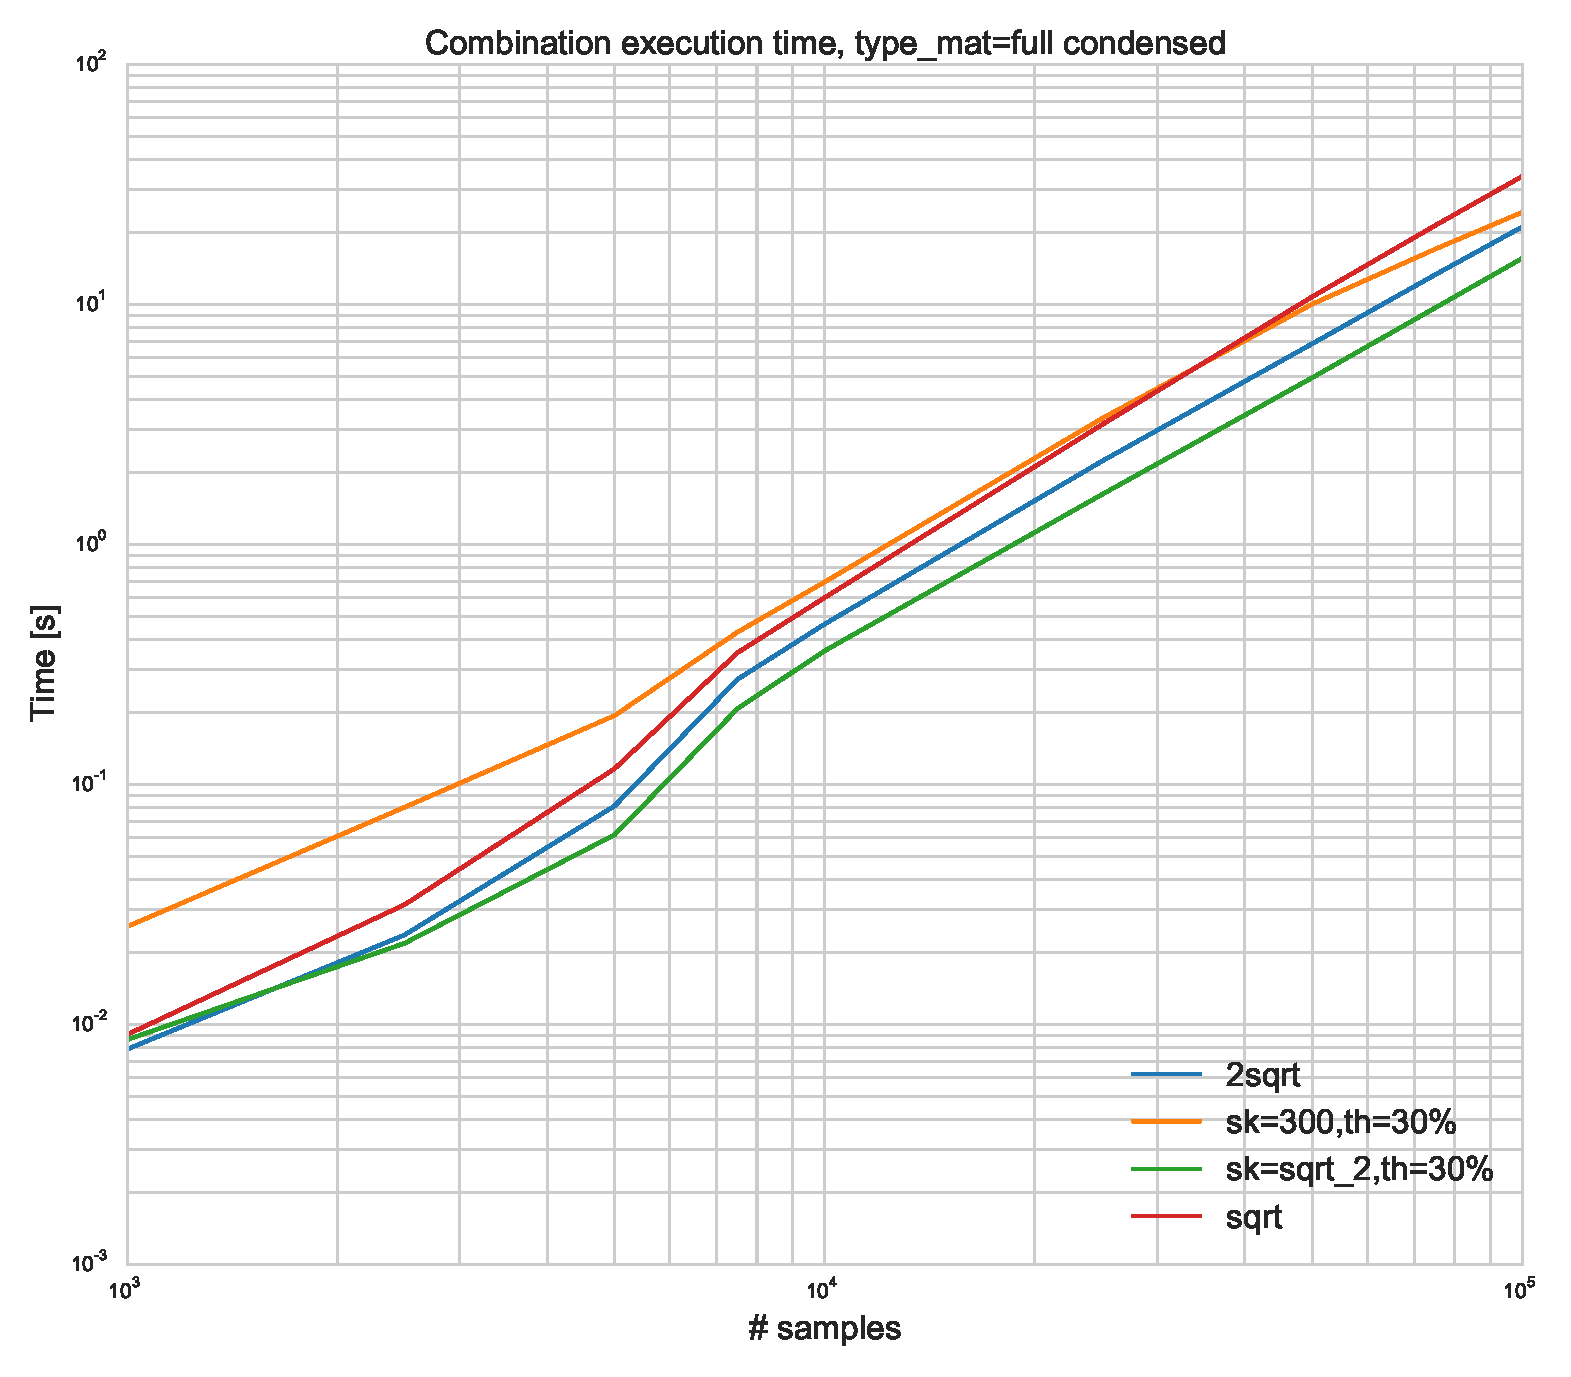
\includegraphics[width=0.6\textwidth]{{{results/eac/sl_mem_time/full_condensed}}}
    \caption{Comparison between the execution times of SLINK to different rules.}
    \label{fig:eac slink}
\end{figure}

\begin{figure}[hbtp]
    \centering
    \includegraphics[width=0.66\textwidth]{{{results/eac/sl_mem_time/sparse_condensed_linear}}}
    \caption{Comparison between the execution times of the three methods of SL over condensed matrices. SLINK runs over fully allocated condensed matrix while SL-MST and SL-MST-Disk run over the sparse matrix.}
    \label{fig:eac sl-mst}
\end{figure}

\subsection{Analysis of the number of associations}

The sparse nature of EAC has been referred to before and is clearer in Fig. \ref{fig:eac assoc density}.
This figure shows the association density, i.e. number of associations relative to the $n^2$ associations in a full matrix.
The \emph{full condensed} format as a constant density of $49.5\%$ and the density of \emph{sparse complete} is two times that of the \emph{sparse condensed} formats.
The overall tendency is for the density to decrease as the number of patterns of the data set increases.
This is to be expected since the \emph{full} matrix grows quadratically.
Besides, it would be expected that the same associations would be grouped together more frequently in partitions and simply previous connections stronger instead of creating new ones.
Results presented in Fig. \ref{fig:eac assocs per pattern}, which presents the number of associations per pattern, suggest otherwise.
The number of associations per pattern increases with the number of patterns of the data set, with the notable exception of the \emph{sk=300} rule which increases until it reaches a certain limit and then stabilizes.
This is explained by the fact that this rule is based on setting a maximum constant number ($300$) of patterns in any given cluster, while in the other rules this number increases with the number of patterns.
The number of patterns per pattern is not $300$ for the $sk=300$ rule because a pattern will be clustered with different neighbors in different partitions.
Still, the number of neighbors doesn't change enough that the number of associations per pattern increases boundlessly.
In fact, Fig. \ref{fig:eac assocs per pattern} suggests that the number of associations per pattern is around 3 times the upper bound on the number of patterns per cluster (strictly related to $K_{min}$).
So, the decrease in density is more related with the quadratic growth of the \emph{full} matrix in contrast with a linear growth of the number of associations.

\begin{figure}[hbtp]
    \centering
    \includegraphics[width=0.6\textwidth]{{{results/eac/assoc_density/sparse_condensed_linear}}}
    \caption{Density of associations relative to the full co-association matrix, which hold $n^2$ associations.}
    \label{fig:eac assoc density}
\end{figure}

\begin{figure}[hbtp]
    \centering
    \includegraphics[width=0.6\textwidth]{{{results/eac/assocs_per_sample}}}
    \caption{Evolution of the total number of associations divided by the number of patterns according to the different rules.}
    \label{fig:eac assocs per pattern}
\end{figure}

Predicting the number of associations before building the co-association matrix is useful for coming up with combination schemes that are both memory and speed efficient.
It was stated before that the biggest cluster size in any partition of the ensemble is a good parameter for this end.
Fig. \ref{fig:eac assocs per pattern} presents the relationship between the biggest cluster size and the maximum number of associations of any pattern.
These ratio increases with the number of patterns in the beginning, but as the number of patterns increases it never goes over 3, which further reinforces the previous statement.

\begin{figure}[hbtp]
    \centering
    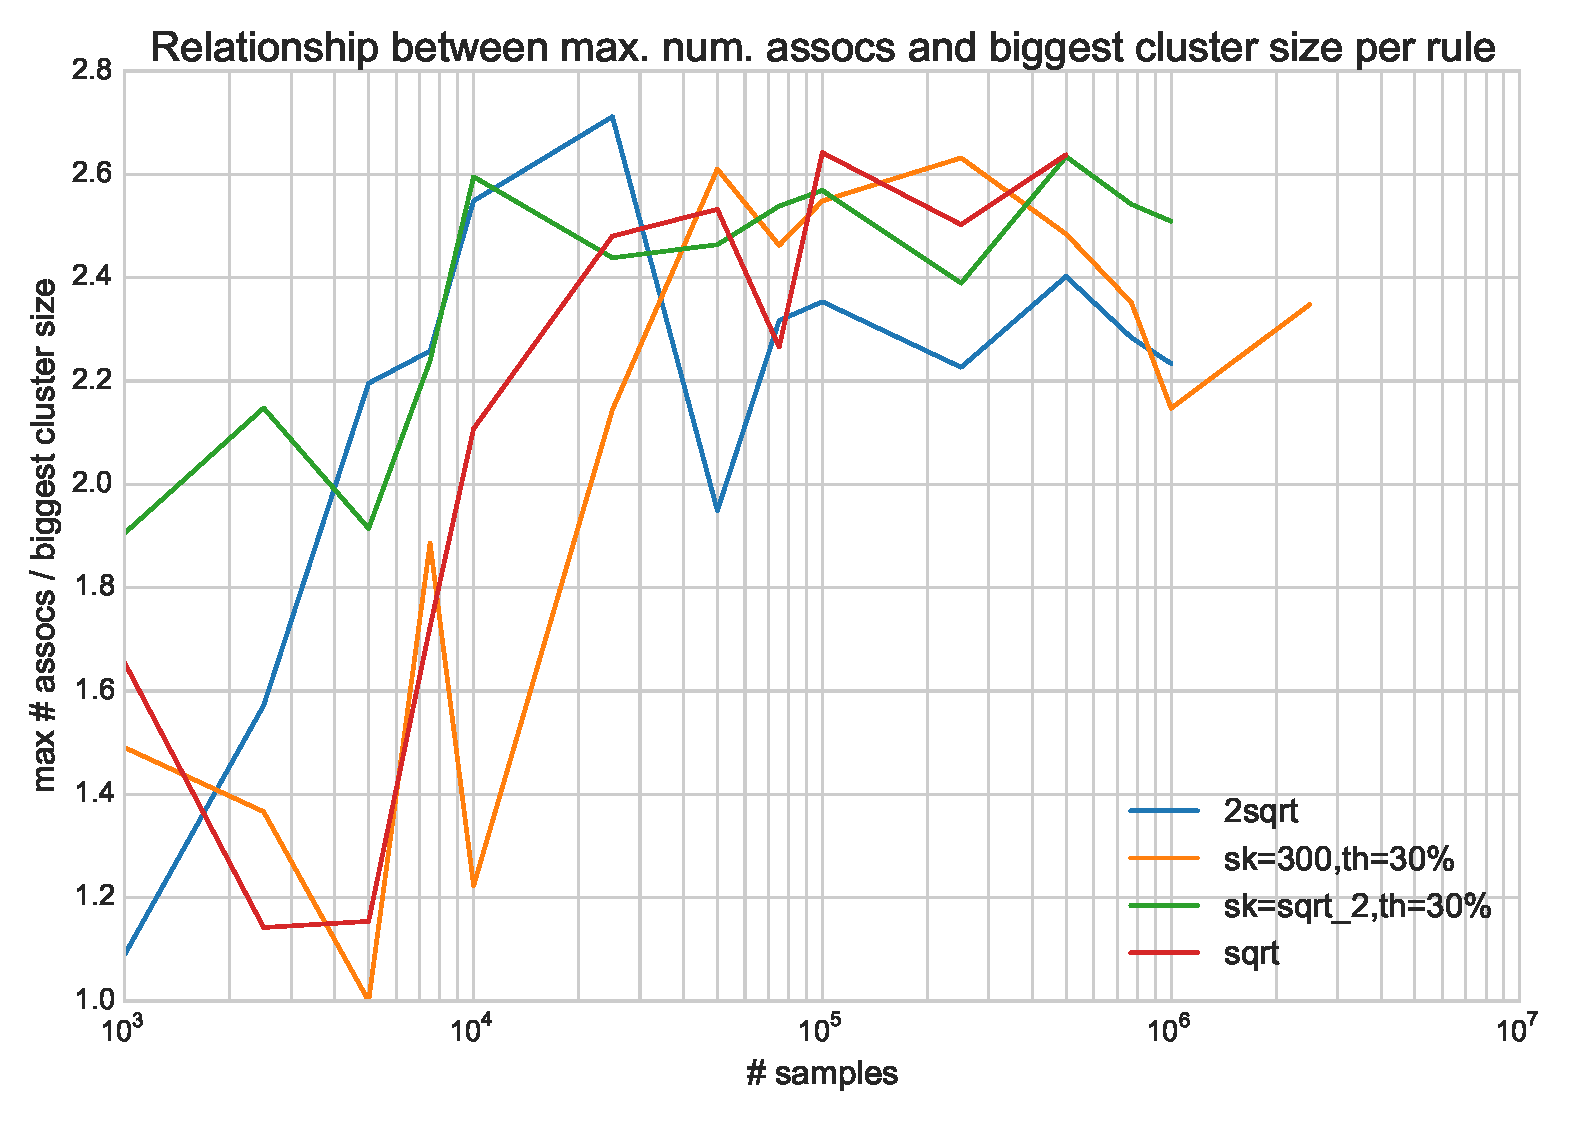
\includegraphics[width=0.6\textwidth]{{{results/eac/max_assoc_bgs}}}
    \caption{Maximum number of associations of any pattern divided by the number of patterns in the biggest cluster of the ensemble.}
    \label{fig:eac assocs per pattern}
\end{figure}

The dimensionality of the used data sets is rather reduced.
One would expect that this ratio would increase with the number of dimensions, since there would be more degrees where the clusters might include other neighbors.
With this in mind, further studies ranging a wider spectrum of data sets should yield more enlightening conclusions or reinforce those presented here.

\subsection{Space complexity}

The previous section analyzed results related to the number of associations.
This is related to the space complexity of the different matrix formats, but does not present an accurate depiction of their complexity.
